\documentclass[conference]{IEEEtran}
\bibliographystyle{IEEEtran}

\usepackage{cite}
\usepackage{amsmath,amssymb,amsfonts}
\usepackage{algorithmic}
\usepackage{graphicx}
\usepackage{textcomp}
\usepackage{xcolor}
\usepackage{lmodern}
\usepackage{minted}
\usepackage{xurl}
\begin{document}

\title{Assembly-Level Implementation of a Minimalist UEFI Bootloader for Custom Operating Systems\\
}

\author{\IEEEauthorblockN{Myint Myat Aung}
\IEEEauthorblockA{\textit{University of Information Technology} \\
Yangon, Myanmar}
}

\maketitle

\begin{abstract}
    This paper presents the implementation of a minimalist UEFI x64 bootloader and kernel entirely in assembly using the FASM assembler.
    The implementation is unique in that both the bootloader and kernel executables are created from simple flat binary output from the assembler. The generation of PE32+ and ELF64 executables and the interfaces required to interact with UEFI hardware are implemented from scratch by referring to their ABI specification documents without relying on libraries.
    This technique eliminates toolchain dependencies, grants full control to the system architect, and facilitates deeper understanding of internal mechanisms.
    The work serves as both a foundation for the future development of a modern operating system free from legacy design decisions and an educational resource for understanding the esoteric nature of operating systems development.
\end{abstract}

\begin{IEEEkeywords}
uefi, bootloader, assembly, operating systems, low-level programming.
\end{IEEEkeywords}

\section{Introduction}
Building an operating system from scratch remains one of the most effective ways to understand how computers truly work.
This paper documents the development of a minimal UEFI bootloader and kernel written entirely in x64 assembly, where every byte of the executable files is crafted by hand.
Unlike typical OS projects that rely on compilers and linkers, this implementation constructs both the bootloader (PE32+ format) and kernel (ELF64 format) through direct assembly programming. Doing this offers complete visibility into the system's lowest levels.

Modern computers begin their startup sequence through a complex interaction between firmware and software. While most developers interact with this process through high-level tools, there's unique value in controlling every aspect:

\begin{itemize}
\item For learners: Manually creating executable files reveals how programs are structured at the binary level.

\item For tinkerers: Handwriting the boot process enables custom behaviors impossible with standard toolchains.

\item For future work: This minimal foundation can grow into a full OS without inheriting unnecessary abstractions.
\end{itemize}

The implementation consists of two core components:

\subsection{A UEFI bootloader}

The UEFI bootloader performs the following:

\begin{itemize}
    \item Prepares the system by calling UEFI functions like ExitBootServices()

    \item Loads the kernel into memory by parsing its ELF64 headers manually

    \item Passes critical hardware information (like the framebuffer) to the kernel
\end{itemize}

\subsection{A demonstration kernel}

The demonstration kernel performs the following:

\begin{itemize}

    \item Takes control from the bootloader

    \item Renders "HELLOWORLD" to the screen by directly manipulating pixels

    \item Uses custom bitmap fonts defined in the assembly code
\end{itemize}

\section{Background}
\subsection{UEFI Overview}

The Unified Extensible Firmware Interface (UEFI) has largely replaced the legacy BIOS as the standard firmware interface for modern computing systems.
UEFI provides a more flexible and modular environment for system initialization, offering features such as secure boot, network booting, and support for larger storage devices.
Unlike BIOS, which operates in 16-bit real mode, UEFI operates in 32-bit or 64-bit protected mode, enabling direct access to modern hardware capabilities.
Bootloaders in UEFI systems are typically implemented as PE32+ executables, which are loaded and executed by the firmware during the boot process. This shift from BIOS to UEFI has introduced new challenges and opportunities in bootloader development, particularly in terms of compatibility. The UEFI boot process is described in Fig.~\ref{uefiboot}. The bootloader to be implemented will serve the purpose of the OS Loader as mentioned in the figure, after the UEFI has loaded all hardware-related devices. This is how UEFI achieves machine-independence.

\begin{figure}[!t]
    \centering
    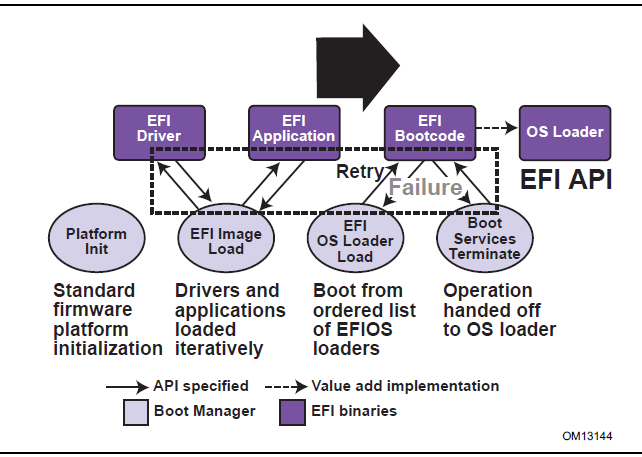
\includegraphics[width=0.9\columnwidth]{uefibootprocess.png}
    \caption{Typical boot process of a UEFI bootloader}
    \label{uefiboot}
\end{figure}

\subsection{PE32+ Binary Format}
The PE32+ (Portable Executable) format is a file format used for executables, object code, and DLLs in Windows and UEFI environments. It includes headers such as the DOS header, PE header, and section headers, which define the executable's structure, entry point, and memory layout. The PE32+ format is essential for UEFI bootloaders, as it ensures compatibility with the firmware's loading mechanism. Similarly, the ELF64 (Executable and Linkable Format) format is widely used for executables in Unix-like operating systems. It includes headers such as the ELF header, program headers, and section headers, which define the executable's memory layout and entry point. The format is further described in Design and Implementation.

\subsection{ELF64 Binary Format}
The ELF64 (Executable and Linkable Format) serves as the standard binary format for 64-bit operating systems and applications \cite{elflatest}, particularly on AMD64/x86-64 architectures. Defined in the System V ABI specification \cite{supplement64}, this format organizes executable code and data into three primary components: (1) the ELF header, which identifies the file type (using the magic sequence 0x7F+'ELF'), specifies the target architecture (0x3E for AMD64), and declares the entry point address where execution begins; (2) program headers that define memory segments with specific permissions (read/write/execute) and loading addresses; and (3) optional section headers for linking and debugging. For AMD64 processors, the format enforces critical architectural requirements including canonical addressing (where upper address bits must be properly sign-extended) and 16-byte stack alignment for function calls. In this project, the kernel's ELF64 structure is manually constructed in assembly, featuring a minimal setup with just two loadable segments: one for executable code (marked with read/execute permissions) loaded at 0x400000, and another for data at 0x600000. This approach provides several advantages over more complex formats like PE32+: it eliminates legacy compatibility fields, allows control over memory layout through straightforward program headers, and maintains portability across Unix-like systems while being simple enough to implement directly in assembly.

\section{Related Work}
There exists other bootloaders that could have been used instead of manually developing one.
\begin{itemize}
    \item GNU GRUB bootloader is by far the most widely used bootloader in the Linux ecosystem. \cite{grub} It has the ability to also load Windows and other OSes and boot manager. While vastly compatible with almost all hardware and software, it is a large and complex bootloader, holding much legacy code and code for backward compatibility. Multiboot 2 is the boot protocol for GRUB \cite{multiboot}, which is used for passing boot-time obtained data to the kernel, but is equally large albeit featureful.
    \item The Limine Bootloader is a modern, advanced, and multiprotocol bootloader. \cite{limine} It supports many architectures including 32-bit x86, x86-64 and arm64 and also supports Multiboot 2. It makes use of the Limine protocol. \cite{limineprotocol}
        This has is origins in hobby OS development but later grew to become usable for other users. 
    \item BOOTBOOT bootloader was created to be minimalistic. \cite{bootboot} It's protocol is the BOOTBOOT Protocol \cite{bootbootprotocol}. Being minimalistic, it does not include features like Secure Boot and dynamic configuration.
\end{itemize}

The bootloader developed is most similar to the BOOTBOOT bootloader, but only focusing on modern x86-64 architectures running on UEFI. This allows it to have a simpler architecture and a solid foundation upon which a modern Operating System can be built without unnecessary legacy compatibility.

\section{Design and Implementation}

The implementation consists of 5 files:

\begin{itemize}
    \item bootloader.asm: Main bootloader FASM source file containing flat binary which will output in the UEFI-compatible PE32+ format, specified according to Microsoft's PE32+ specification \cite{pe}
    \item kernel.asm: Source FASM file of the demo kernel containing flat binary which will output in the ELF64 format, specified according to ELF64 specification \cite{elflatest}. The rationale behind choosing ELF64 is due to being widely used in the Linux, being field-tested, and the relatively simple structure of the binary.
    \item bootloaderstruct.inc: Custom defined structures to use when passing information about the system environment that the bootloader gathered to the kernel. Currently only supports passing graphics information. A standard can be defined later.
    \item elf.inc: Manually defined ELF64 structures so that the bootloader can parse them. Defined according to ELF \cite{elflatest} and AMD64 processor-specific \cite{supplement64} specification documents
    \item efi.inc: Manually defined EFI structures for interacting with UEFI firmware to perform tasks like getting memory map, printing to screen, allocating disk space, etc. Defined according to UEFI specifications \cite{uefi}.
\end{itemize}


UEFI-specific structures, such as the System Table, were defined based on the UEFI specification. These structures facilitated interaction with UEFI services, including getting memory map, printing to the screen, memory allocation and boot services termination.

The process is as follows:

\begin{itemize}
    \item The bootloader is loaded into memory as an UEFI application by the UEFI firmware of the machine that it is running on (whether it be virtual or physical).
    \item The bootloader outputs to the screen its status using the defined UEFI functions from the system table.
    \item The bootloader loads the kernel file in the file system into memory
    \item The bootloader parses the kernel file according to the ELF64 format, discovering information about the size of the kernel, etc.
    \item The bootloader gets the memory map of the system used to change execution environment.
    \item The bootloader passes arguments using bootloaderstruct.inc, passes execution control to the kernel and jumps to the kernel entry point.
    \item The kernel code begins execution, performing boot up of the operating system.
\end{itemize}

The following snippet \ref{snippetefi} describes the System Table and Table header structures, amongst others, as defined in the UEFI specs. They are the main functions the bootloader must use to load a kernel.

\begin{listing}[!t]
    \inputminted[breaklines,breakanywhere,frame=single]{nasm}{snippetefi.asm}
    \caption{EFI system table and table header structures required to interface with UEFI, amongst other structures}
    \label{snippetefi}
\end{listing}

The flat binary output is produced using code such as in \ref{snippetkernel}, where assembly "define byte" and family directives are used.

\begin{listing}[!t]
    \inputminted[breaklines,breakanywhere,frame=single]{nasm}{snippetkernel.asm}
    \caption{Kernel ELF EHeader defined using define byte primitives according to ELF specification}
    \label{snippetkernel}
\end{listing}

UEFI function calls are performed using Microsoft x64 calling convention in assembly as defined in the specifications \cite{microsoftx64calling}.

The process of loading the kernel file into memory is described in \ref{snippetvolume}. This involves using the UEFI OpenVolume function, a part of BootServices which give full functionality for OS loaders.

\begin{listing}[!t]
    \inputminted[breaklines,breakanywhere,frame=single]{nasm}{snippetvolume.asm}
    \caption{Discovering the volume in which the kernel file is situated and loading it into memory}
    \label{snippetvolume}
\end{listing}

The loaded exceutable is parsed using the ELF structure as in \ref{snippetelf}.

\begin{listing}[!t]
    \inputminted[breaklines,breakanywhere,frame=single]{nasm}{snippetelf.asm}
    \caption{ELF64 EHeader and Program Header structures, amongst other structures}
    \label{snippetelf}
\end{listing}

\ref{snippetexit} marks the important execution transfer point, where the bootloader gathers memory map information, loads it up as arguments to the kernel and passes execution to the kernel. Arguments are passed using the bootloaderstruct structure defined in \ref{snippetbootloaderstruct}.

\begin{listing}[!t]
    \inputminted[breaklines,breakanywhere,frame=single]{nasm}{snippetexit.asm}
    \caption{The entry point: Getting memory map, exiting boot services and passing arguements and passing execution from bootloader to kernel}
    \label{snippetexit}
\end{listing}

\begin{listing}[!t]
    \inputminted[breaklines,breakanywhere,frame=single]{nasm}{snippetbootloaderstruct.asm}
    \caption{Custom bootloader structure used to pass information from bootloader to kernel}
    \label{snippetbootloaderstruct}
\end{listing}

\ref{snippetkernelargs} is where the kernel obtains the information passed to it. and saves the arguments.

\begin{listing}[!t]
    \inputminted[breaklines,breakanywhere,frame=single]{nasm}{snippetkernelargs.asm}
    \caption{Receiving kernel arguments from the bootloader using bootloaderstruct}
    \label{snippetkernelargs}
\end{listing}

This completes the bootloading and kernel execution process.

\section{Results}

For the purposes of testing, the bootloader and kernel can be copied to into an EFI-compatible image and then transformed into a bootable ISO. The Makefile displayed in \ref{snippetmakefile} is used to automate the process of:

\begin{itemize}
    \item Assembling the bootloader and kernel source
    \item Creating an empty EFI compatible image
    \item Creating an EFI compatible ISO from said image using xorriso
    \item Creating and running the virtual machine with said ISO as the medium
\end{itemize}

\begin{listing}[!t]
    \inputminted[breaklines,breakanywhere,frame=single]{nasm}{snippetmakefile.txt}
    \caption{Makefile used to create and run the virtual machine}
    \label{snippetmakefile}
\end{listing}

When run using the Linux QEMU emulator, the virtual machine boots up and successfully renders the letters 'HELLOWORLD', as can be seen in \ref{screenshot}.

\begin{figure}[!t]
    \centering
    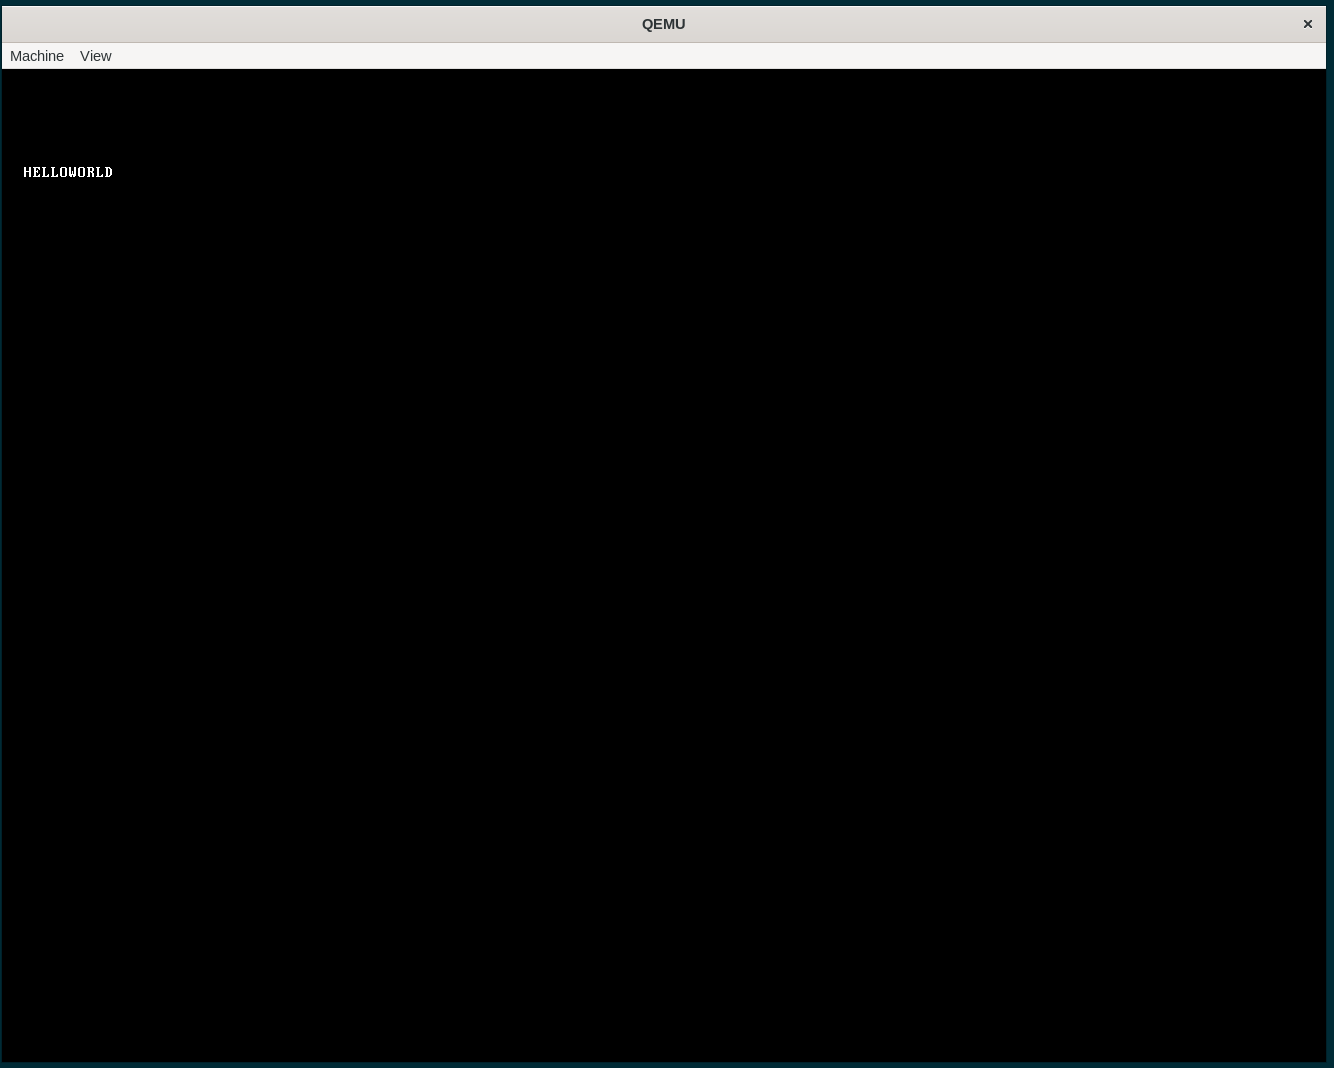
\includegraphics[width=0.9\columnwidth]{screenshot.png}
    \caption{Bootloader successfully loading the demo kernel inside QEMU}
    \label{screenshot}
\end{figure}

\section{Discussion}
The implementation of this UEFI bootloader represents a significant milestone in the ongoing effort to develop a custom operating system. \cite{elflatest}


The reason for the development of the bootloader implementation as described in this paper is to serve as the foundation for a modern operating system which is minimal in nature and does not contain "legacy baggage". Legacy baggage consists of (but is not limited to) the following:

\begin{itemize}
    \item Outdated Design Decisions
    \item Accumulation of legacy code
    \item The need to maintain backward compatibility
\end{itemize}

\subsection{Outdated Design Decisions}
Two of the most widely used operating systems currently, Windows and Linux-based distributions, were first released in 1991 and 1985 respectively.
The design decisions made during the development of these OSes were based on outdated assumptions.
An example is UNIX (which Linux is based on) was initially created for allowing multiple users to simultaneously use a single large mainframe via terminals.
For this, UNIX offers multiuser sessions and terminal multiplexing.
Linux also sets these virtual terminals up when the computer is booted up, and exposes multiple tty devices.
In the modern day, desktop OSes are used mostly by a single user.
It would be desirable to simplify this by only using one terminal, or even wholly eliminating the concept of the terminal (terminal as in the device and not the command-line interface).
Doing so would bring about a small performance gain but most importantly make the OS's architecture simpler, allowing codebase maintenance to be easier.

\subsection{Accumulation of legacy code}

This is the issue of old code accumulating over the course of decades of development.
This can amount to millions of lines of code, degrading performance and increasing the rate of failures, a phenomenon often referred to as Software aging.
Linux is not an exception and analysis of the Linux kernel's aging codebase has been carried out by others. \cite{linuxaging, linuxaging2}
The sheer size of these codebases require a huge undertaking to refactor.

\subsection{The need to maintain backward compatibility}

This refers to the maintaining of code solely due to support old hardware or software technologies. e.g UEFI is replacing BIOS in almost all modern computers. Both Windows and Linux distributions need to support old BIOS plaforms in order that they keep running on legacy hardware. Another example is 32-bit x86 code. x86-64 (the 64-bit architecture) has superceded 32-bit x86, which could only support 2 GB of RAM. An OS focused on modern hardware need not maintain backward compatibility with BIOS and 32-bit architecture. A side effect in addition to simplifying architecture is that security is vastly improved as there is a smaller attack surface.

A possible future operating system could be a multi-kernel approach like the Barrelfish OS described by Baumann et al. in \cite{barrelfish}. This kind of OS allows massive parallelization and scalability as it is distributed in the lowest kernel level instead of using a middleware to achieve distributed properties. Future work may be based on such a kernel.

\section{Conclusion}
This paper presented the implementation of a minimalist UEFI bootloader developed entirely in assembly.
The bootloader UEFI (PE32+) application successfully loads a custom ELF64 kernel that displays 'HELLOWORLD'.
The system implements the UEFI, System V ELF ABI and PE32+ executable standards to build interfaces that allow communication with the hardware, eliminating the use of external libraries and thus keeping the source minimal and easy-to-understand.

The project represents a critical first step in the broader effort to develop a custom modern operating system, free from legacy architecture and unnecessary backward compatibilities.
Future work will build on this foundation, extending the bootloader and integrating it with other components of the operating system.
The minimalistic nature of the implementation allows it to be used as an education resource in Operating Systems curriculums to offer clear insight into the practical, low-level workings of a bootloaders's mechanisms.

The implementation is available on Github at \cite{mygithub}. 

\section*{Acknowledgment}

The author expresses deepest gratitude to all current and past Professors of the High-Performance Computing major at the University of Information Technology who have, over the course of two academic years, shared their knowledge and offered their exceptional guidance and encouragement. Their profound ability to deliver concepts during lectures demystified complex concepts and laid the foundation for this work. Special thanks to the Department of Computer Science and the institute for providing the environment and facilities that made this paper possible.

\bibliography{IEEEabrv,references}

\end{document}
